\documentclass[mathserif,serif]{beamer}
\usetheme{Madrid}
\usecolortheme{seagull}

\usepackage{graphicx}
\usepackage{listings}

\newenvironment{items}{
\begin{itemize}
  \setlength{\itemsep}{0pt}
  \setlength{\parskip}{7pt}
  \setlength{\parsep}{4pt}
}{\end{itemize}}

\begin{document}

\begin{frame}[t]
    \frametitle{About Me}

    \begin{items}
        \item Elvis Flesborg

        \item Master thesis on ITU Copenhagen
        \item Claus Brabrand as supervisor
        \item Jean Melo as co-supervisor
    \end{items}
\end{frame}

\begin{frame}[t]{About the Project}
    

    \begin{items}
        \item Make a representative sample of all configurations.
        \item Look for errors in them.
        \begin{items}
            \item If too few are found, scale down to warnings.
        \end{items}
    \end{items}

    
    Answer questions like:
    

    \begin{items}
        \item How many bugs are there in total?
        \item What types of bugs are there most of?
        \item Where are the bugs mostly located?
        \item ... more?
    \end{items}
\end{frame}

\begin{frame}[t]{About the Linux Kernel}
    

    \begin{items}
        \item 14172 different features \footnote{ grep }.
        \item That is $2^{14172}$ different configurations.
        \item Still more than estimated number of atoms in the known universe.
        \item Will use the already existing tool \emph{make randconfig}.
    \end{items}
\end{frame}

\begin{frame}[t]
    
    \frametitle{The Sample}
    

    It is important to get a representative sample

    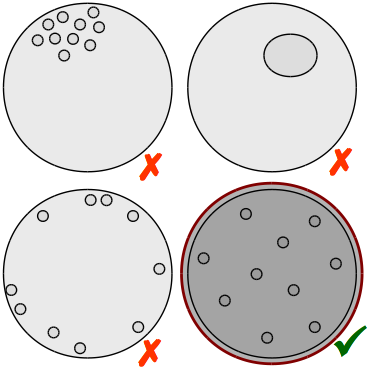
\includegraphics[scale=.5]{sample.png}
\end{frame}

\begin{frame}[t]{Compiling a Linux Kernel}

    \begin{items}
        \item `make randconfig` - create a random configuration.
        \item `make` - compile the Linux Kernel.
        \item Save all kinds of information about the compilation.
        \begin{items}
            \item Errors / warnings.
            \item Configuration.
        \end{items}
        \item Do it over and over again.
        \item Take cross-compiling into account.
    \end{items}


\end{frame}

\begin{frame}[t]{Kconfig}

    \begin{items}
        \item The language of the configurations.
        \begin{items}
            \item Data types
            \item Dependencies
            \item Menu structure (irrelevant to this project)
        \end{items}


    Example code, and explaination will be given.
    \end{items}
\end{frame}

\begin{frame}[t,fragile]{Kconfig - Grammar}
    \begin{lstlisting}
K ->      'config' ID TYPE OPTS
        | 'menuconfig' ID
        | 'if' ID K 'endif'
        | 'choice' K K+ 'endchoice'
        | 'menu' STRING K 'endmenu'

TYPE ->   'bool' | 'tristate' | 'string' | 'int'

OPTS ->   'default' STRING
        | 'help' STRING
        | 'range' INT
        | 'depends on' ID
        | 'select' ID
    \end{lstlisting}
\end{frame}

\begin{frame}[t,fragile]{Kconfig - Data types}
    \begin{columns}[T]
    \column{.5\textwidth}
    \begin{lstlisting}
config A
    bool
config B
    tristate
config C
    int
    range 5 15
config D
    hex
    default "c0000000"
config E
    string
    default "FOO"
    \end{lstlisting}
    \column{.5\textwidth}
    \begin{lstlisting}

yes, no (tristate)

yes, no, module

integers (string)


hexadecimals (string)


string
    \end{lstlisting}
    \end{columns}
\end{frame}

\begin{frame}[t,fragile]{Kconfig - Dependencies example}
    \begin{columns}[t]
    \column{.4\textwidth}
    \begin{lstlisting}
config A
    bool

config B
    bool
    depends on A

config C
    bool
    depends on A
    \end{lstlisting}

    \column{.2\textwidth}
    \textbf{Same as}

    \column{.4\textwidth}
    \begin{lstlisting}
config A
    bool

if A
    config B
        bool
    
    config C
        bool
endif
    \end{lstlisting}
    \end{columns}
\end{frame}

\begin{frame}[t,fragile]{Kconfig - Dependencies explaination}

    \begin{columns}[T]
    \column{.4\textwidth}
    \begin{lstlisting}
config B
    bool
    depends on A

config A
    bool
    \end{lstlisting}
    \column{.6\textwidth}
    \begin{items}
        \item B can only be enabled if \emph{A} is enabled.
        \item `make randconfig` will roll a dice for \emph{A} first because it 
                is a dependency.
        \item Will not just autoselect \emph{A}. We have `select` for that.
    \end{items}

    \end{columns}
    
\end{frame}

\begin{frame}[t]{Kconfig}

    \begin{columns}[T]
    \column{.4\textwidth}

    \begin{lstlisting}

    \end{lstlisting}

    \column{.6\textwidth}

    \begin{items}
        \item
    \end{items}

    \end{columns}
\end{frame}

\end{document}
